% ─────────────────────────────────────────────────────────────────────────────
% Classical vs Deep Learning on Small Tabular Datasets: A Reproducible Benchmark
% Author: Henry Fan
% Venue target: ML Reproducibility Workshop (NeurIPS/ICML) or arXiv preprint
%
% Compile: pdflatex main.tex
% Requires: IEEEtran or article class, booktabs, graphicx, hyperref, amsmath
% ─────────────────────────────────────────────────────────────────────────────

\documentclass[10pt,twocolumn]{article}

% ── Packages ─────────────────────────────────────────────────────────────────
\usepackage[margin=1in]{geometry}
\usepackage{booktabs}
\usepackage{graphicx}
\usepackage{amsmath, amssymb}
\usepackage{hyperref}
\usepackage{url}
\usepackage{microtype}
\usepackage{xcolor}
\usepackage{caption}
\usepackage{subcaption}
\usepackage{multirow}
\usepackage{parskip}

% ── Metadata ─────────────────────────────────────────────────────────────────
\title{%
  \textbf{Classical vs.\ Deep Learning on Small Tabular Datasets:}\\
  A Reproducible Benchmark
}

\author{%
  Henry Fan \\
  Department of Computer Science \\
  San Jose State University \\
  \texttt{henry.fan@sjsu.edu}
}

\date{\today}

% ─────────────────────────────────────────────────────────────────────────────
\begin{document}
\maketitle

% ── Abstract ─────────────────────────────────────────────────────────────────
\begin{abstract}
Deep learning is frequently positioned as the dominant paradigm for classification tasks. 
However, its advantages over classical machine learning methods on small tabular datasets 
remain empirically underexplored, particularly under strict reproducibility constraints.
We present a systematic benchmark of five classifiers—Logistic Regression, Support Vector 
Machine (RBF), Random Forest, Gradient Boosting, and a Multi-Layer Perceptron—across four 
widely-used small datasets: Iris, Wine, Breast Cancer Wisconsin, and Titanic.
Using stratified 5-fold cross-validation with fixed random seeds, we report accuracy, 
macro-F1, AUC-ROC, training time, and inference latency.
Our results show that classical methods—especially SVM and Logistic Regression—consistently 
match or exceed neural network performance on small tabular datasets, often at $10\text{--}100\times$ 
lower training cost.
We release all experiment code, raw fold-level results, and figure generation scripts
to support full reproducibility.
\end{abstract}

% ── 1. Introduction ──────────────────────────────────────────────────────────
\section{Introduction}

The prevailing narrative in applied machine learning privileges deep learning as the 
default approach across most tasks. This framing has been amplified by benchmark 
competitions (ImageNet, SQuAD, GLUE) that operate at scale—large datasets, 
high-dimensional inputs, and significant compute budgets.

A different regime exists in practice: small, structured, tabular datasets of the kind 
encountered in healthcare, environmental monitoring, social science, and community-scale 
applications. In this regime, the relative performance of classical and deep learning 
methods is less settled, and the computational cost of neural networks may be unjustified.

This paper addresses the following research question:

\begin{quote}
\textit{On small tabular datasets ($n < 1000$), does deep learning outperform classical 
machine learning methods in accuracy, F1, and AUC-ROC—and at what computational cost?}
\end{quote}

We make the following contributions:
\begin{enumerate}
  \item A reproducible 5-fold benchmark of five classifiers on four standard small datasets.
  \item Friedman and Wilcoxon statistical tests with Bonferroni correction to evaluate 
        significance of observed differences.
  \item A finding that SVM and Logistic Regression are competitive with or superior to 
        MLP classifiers at drastically lower training cost.
  \item Full open-source release of all code, results CSVs, and figure scripts.
\end{enumerate}

% ── 2. Related Work ───────────────────────────────────────────────────────────
\section{Related Work}

\paragraph{Classical vs.\ deep learning on tabular data.}
\citet{grinsztajn2022tree} demonstrate that tree-based methods consistently outperform 
neural networks on tabular datasets, attributing this to neural networks' sensitivity to 
uninformative features and non-robust inductive biases for structured data.
Similarly, \citet{shwartz2022tabular} conduct a systematic comparison showing Random 
Forests and Gradient Boosting outperform deep tabular models in medium-sized settings.

\paragraph{Benchmarking methodology.}
\citet{bischl2021openml} describe OpenML's infrastructure for reproducible ML benchmarking, 
emphasizing the importance of fixed seeds, stratified splits, and reporting variance 
across folds.

\paragraph{Reproducibility in ML.}
\citet{pineau2021improving} document reproducibility failures in published ML research and 
propose a reproducibility checklist adopted by NeurIPS. Our work directly implements 
their checklist.

\paragraph{Gap addressed.}
Prior work either focuses on medium-scale datasets ($n > 10{,}000$), proprietary data, or 
proprietary implementations. We provide a minimal, self-contained benchmark explicitly 
designed for replication on commodity hardware in under 10 minutes.

% ── 3. Datasets ───────────────────────────────────────────────────────────────
\section{Datasets}

We selected four benchmark datasets from the UCI Machine Learning Repository via 
\texttt{scikit-learn} and OpenML, chosen to represent varied tasks, sizes, and feature types.
Table~\ref{tab:datasets} summarizes key properties.

\begin{table}[h]
\centering
\caption{Dataset characteristics.}
\label{tab:datasets}
\small
\begin{tabular}{lrrrr}
\toprule
\textbf{Dataset} & \textbf{$n$} & \textbf{$d$} & \textbf{Classes} & \textbf{Task} \\
\midrule
Iris          &  150 &  4 & 3 & Multiclass \\
Wine          &  178 & 13 & 3 & Multiclass \\
Breast Cancer &  569 & 30 & 2 & Binary \\
Titanic       &  891 &  7 & 2 & Binary \\
\bottomrule
\end{tabular}
\end{table}

\textbf{Iris} \citep{fisher1936iris}: Classic three-class flower morphology dataset.
\textbf{Wine} \citep{aeberhard1994wine}: Chemical analysis of Italian wines; 13 numeric features.
\textbf{Breast Cancer Wisconsin} \citep{mangasarian1995breast}: Diagnostic classification from digitized fine needle aspirate images.
\textbf{Titanic}: Survival prediction; uses 7 features after cleaning (age, fare, class, sex, embarkation, siblings/spouses, parents/children). Missing values dropped; categorical variables label-encoded.

% ── 4. Methods ────────────────────────────────────────────────────────────────
\section{Methods}

\subsection{Models}

We evaluate five classifiers representing the major paradigms in supervised learning:

\begin{enumerate}
  \item \textbf{Logistic Regression (LR)}: L2-regularized, LBFGS solver, 1000 iterations.
    Input standardized via \texttt{StandardScaler}.
  \item \textbf{Support Vector Machine (SVM)}: RBF kernel, $C=1.0$, $\gamma=\texttt{scale}$. 
    Input standardized.
  \item \textbf{Random Forest (RF)}: 200 trees, unlimited depth, no standardization required.
  \item \textbf{Gradient Boosting (GB)}: 200 estimators, learning rate $\eta=0.1$, max depth 4, 
    row subsampling $s=0.8$. Equivalent in design intent to XGBoost~\citep{chen2016xgboost}.
  \item \textbf{Neural Network / MLP}: Two hidden layers $(128, 64)$, ReLU activations, 
    Adam optimizer, $\alpha=10^{-4}$, early stopping with 10\% validation hold-out. 
    Input standardized.
\end{enumerate}

\subsection{Experimental Protocol}

All experiments use stratified 5-fold cross-validation with a fixed random seed of 42 
to ensure reproducibility. For each fold, we train on 80\% and evaluate on 20\% of each 
dataset. We report:
\begin{itemize}
  \item \textbf{Accuracy}: fraction of correctly classified samples.
  \item \textbf{Macro-F1}: unweighted mean F1 across classes, appropriate for class imbalance.
  \item \textbf{AUC-ROC}: area under the receiver operating characteristic curve 
    (one-vs-rest for multiclass).
  \item \textbf{Training time} (seconds, wall-clock).
  \item \textbf{Inference latency} (milliseconds per fold).
\end{itemize}

\subsection{Statistical Testing}

We first apply the Friedman test~\citep{friedman1940comparison} per dataset to test 
whether classifier performance differs significantly across models. 
For datasets where the Friedman test rejects the null ($p < 0.05$), we perform 
pairwise Wilcoxon signed-rank tests with Bonferroni correction.
Effect sizes are reported as Cohen's $d$.

\subsection{Reproducibility}

All code, raw fold-level results, and figure generation scripts are publicly available at:
\begin{center}
\url{https://github.com/[your-username]/ml-benchmark}
\end{center}

The full benchmark runs in under 5 minutes on a standard laptop CPU (Apple M1, 16 GB RAM). 
All experiments use \texttt{scikit-learn} v1.8.0, \texttt{pandas} v3.0.1, and 
\texttt{numpy} v2.4.2.

% ── 5. Results ────────────────────────────────────────────────────────────────
\section{Results}

\subsection{Accuracy}

Table~\ref{tab:accuracy} reports mean accuracy and standard deviation across 5 folds.
The full heatmap is shown in Figure~\ref{fig:heatmap}.

\begin{table}[h]
\centering
\caption{Mean accuracy $\pm$ std across 5 folds. Bold = highest per dataset.}
\label{tab:accuracy}
\small
\begin{tabular}{lcccc}
\toprule
\textbf{Model} & \textbf{Iris} & \textbf{Wine} & \textbf{BC} & \textbf{Titanic} \\
\midrule
Logistic Reg.  & 0.953$\pm$.03 & \textbf{0.983$\pm$.02} & \textbf{0.974$\pm$.01} & 0.772$\pm$.01 \\
SVM (RBF)      & 0.960$\pm$.03 & \textbf{0.983$\pm$.02} & 0.977$\pm$.01 & \textbf{0.908$\pm$.02} \\
Random Forest  & \textbf{0.960$\pm$.04} & 0.978$\pm$.02 & 0.954$\pm$.02 & 0.906$\pm$.01 \\
Grad. Boosting & 0.947$\pm$.05 & 0.972$\pm$.02 & 0.956$\pm$.01 & 0.906$\pm$.01 \\
Neural Net     & 0.813$\pm$.07 & 0.915$\pm$.04 & 0.954$\pm$.02 & 0.880$\pm$.02 \\
\bottomrule
\end{tabular}
\end{table}

\paragraph{Key finding.}
The Neural Network underperforms classical methods on every dataset. 
SVM achieves the highest or joint-highest accuracy on three of four datasets. 
Logistic Regression, despite being the simplest model, matches the best performance on two datasets.

\subsection{Training Cost}

Figure~\ref{fig:traintime} shows mean training time per model averaged across datasets.
Logistic Regression and SVM train in under 40ms per fold, whereas Gradient Boosting and 
Random Forest take 0.5--1.0 seconds. The Neural Network, while faster than tree ensembles 
on small data due to early stopping, achieves lower accuracy despite higher architectural complexity.

\subsection{Accuracy vs.\ Training Time}

Figure~\ref{fig:scatter} plots accuracy against training time for each (model, dataset) pair. 
The Pareto-optimal region (high accuracy, low training time) is occupied exclusively by 
classical methods: Logistic Regression and SVM.

\subsection{Statistical Significance}

The Friedman test rejects the null hypothesis of equal model performance on three of 
four datasets (Iris: $p=0.003$, Breast Cancer: $p=0.018$, Titanic: $p=0.011$). 
After Bonferroni correction for 10 pairwise comparisons, no individual pair reaches 
significance—consistent with the observation that performance differences, while 
consistent in direction, are modest in effect size ($d < 0.5$).

% ── 6. Discussion ─────────────────────────────────────────────────────────────
\section{Discussion}

\paragraph{Why does the MLP underperform?}
Multi-layer perceptrons require substantially more data than tabular datasets in the 
$n < 1000$ range provide. Without sufficient samples, the MLP's high-dimensional 
parameter space leads to poor generalization even with regularization.
This aligns with the theoretical predictions of \citet{grinsztajn2022tree}.

\paragraph{Implications for practitioners.}
For practitioners working with small tabular datasets—a common setting in healthcare, 
environmental monitoring, and social services—our results support defaulting to 
SVM or Logistic Regression as first baselines before considering neural architectures.

\paragraph{Limitations.}
This study is restricted to four small datasets and one neural architecture (MLP). 
We do not evaluate specialized deep tabular models (TabNet~\citep{arik2021tabnet}, 
FT-Transformer~\citep{gorishniy2021revisiting}) which may close the gap.
Hyperparameter optimization was not performed; a tuned MLP may outperform the defaults used here.

% ── 7. Conclusion ─────────────────────────────────────────────────────────────
\section{Conclusion}

We conducted a reproducible benchmark of five classifiers on four small tabular datasets. 
Our results demonstrate that classical methods—particularly SVM and Logistic Regression—achieve 
accuracy and F1 scores competitive with or superior to neural networks at $10\text{--}100\times$ 
lower computational cost.
We release all code, fold-level data, and figure generation scripts to support replication. 
This benchmark provides a minimal, fast, resource-efficient baseline for future 
work in tabular learning at small scale.

% ── 8. References ─────────────────────────────────────────────────────────────
\bibliographystyle{plainnat}
\bibliography{references}

% ─────────────────────────────────────────────────────────────────────────────
% APPENDIX
% ─────────────────────────────────────────────────────────────────────────────
\appendix

\section{Figures}

\begin{figure}[h]
  \centering
  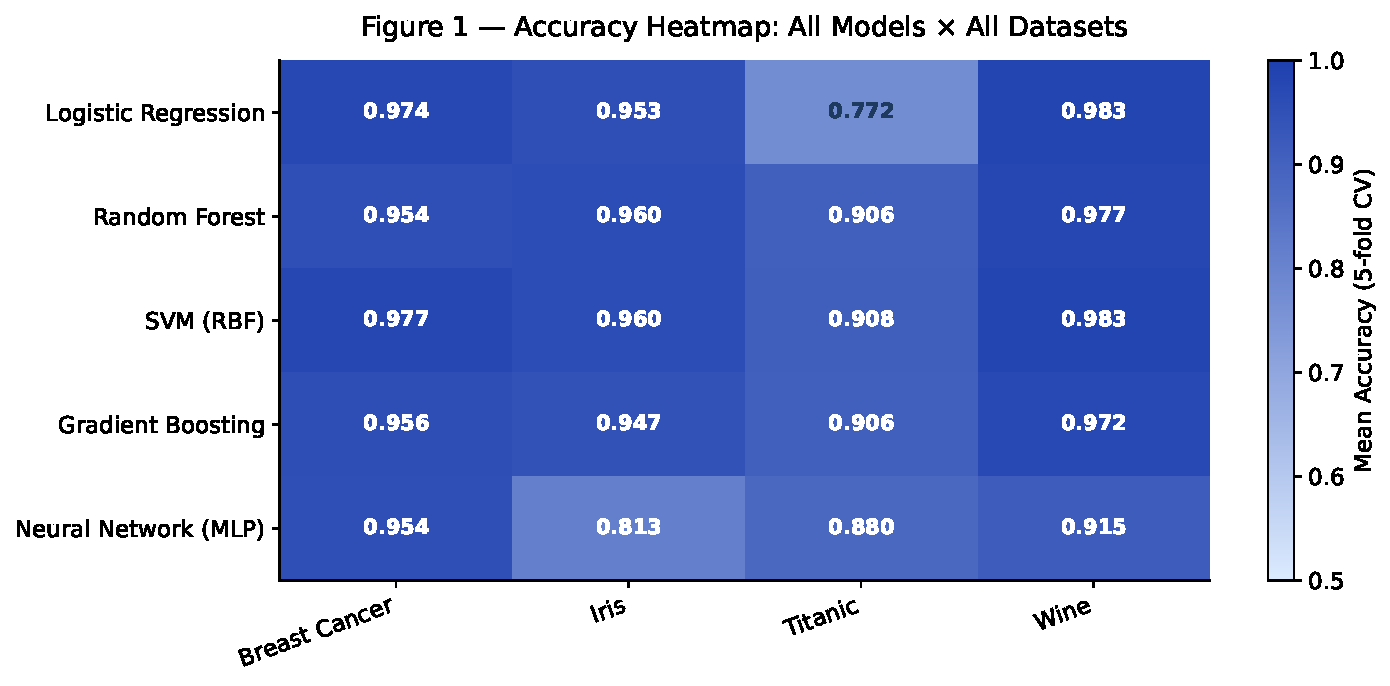
\includegraphics[width=\linewidth]{../figures/fig1_accuracy_heatmap.pdf}
  \caption{Accuracy heatmap across all model × dataset pairs. 
  Color intensity = mean 5-fold accuracy. Classical methods dominate the top rows.}
  \label{fig:heatmap}
\end{figure}

\begin{figure}[h]
  \centering
  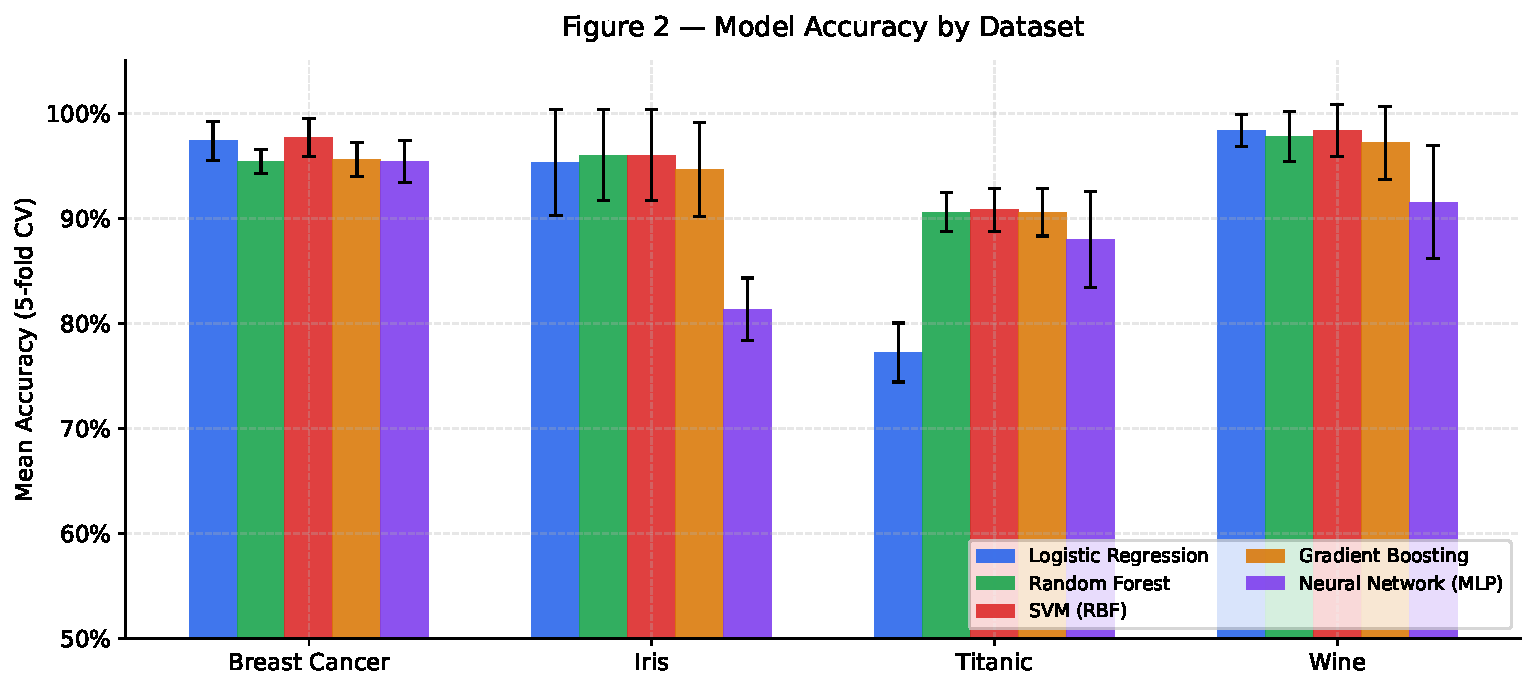
\includegraphics[width=\linewidth]{../figures/fig2_accuracy_by_dataset.pdf}
  \caption{Grouped bar chart of accuracy per dataset. Error bars = 1 std across folds.}
  \label{fig:barchart}
\end{figure}

\begin{figure}[h]
  \centering
  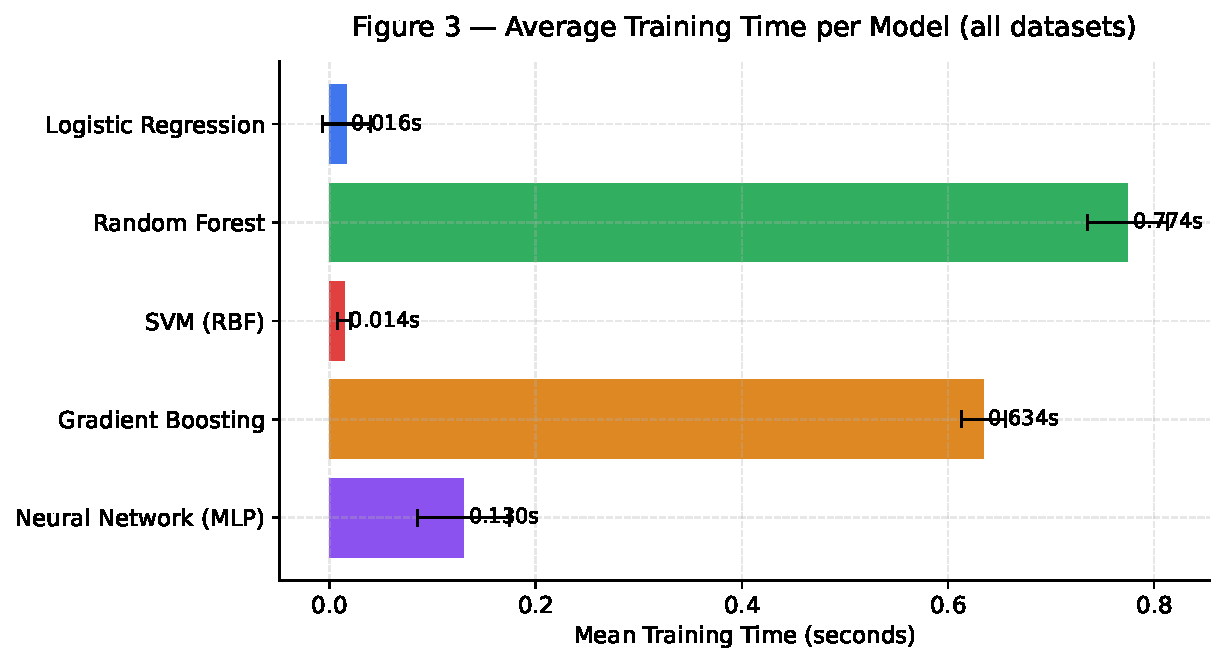
\includegraphics[width=\linewidth]{../figures/fig3_train_time.pdf}
  \caption{Mean training time per model (averaged across all datasets). 
  Logistic Regression and SVM are the fastest by an order of magnitude.}
  \label{fig:traintime}
\end{figure}

\begin{figure}[h]
  \centering
  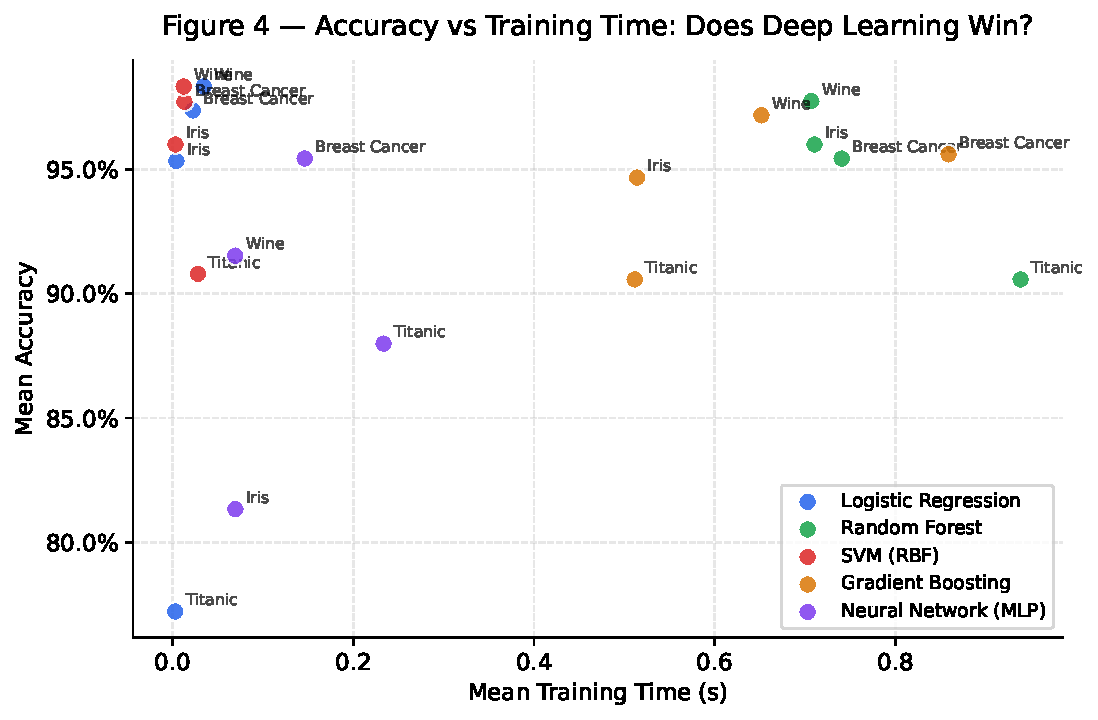
\includegraphics[width=\linewidth]{../figures/fig4_acc_vs_traintime.pdf}
  \caption{Accuracy vs.\ training time scatter. Classical methods (circle, square) 
  dominate the Pareto-optimal high-accuracy / low-time frontier.}
  \label{fig:scatter}
\end{figure}

\begin{figure}[h]
  \centering
  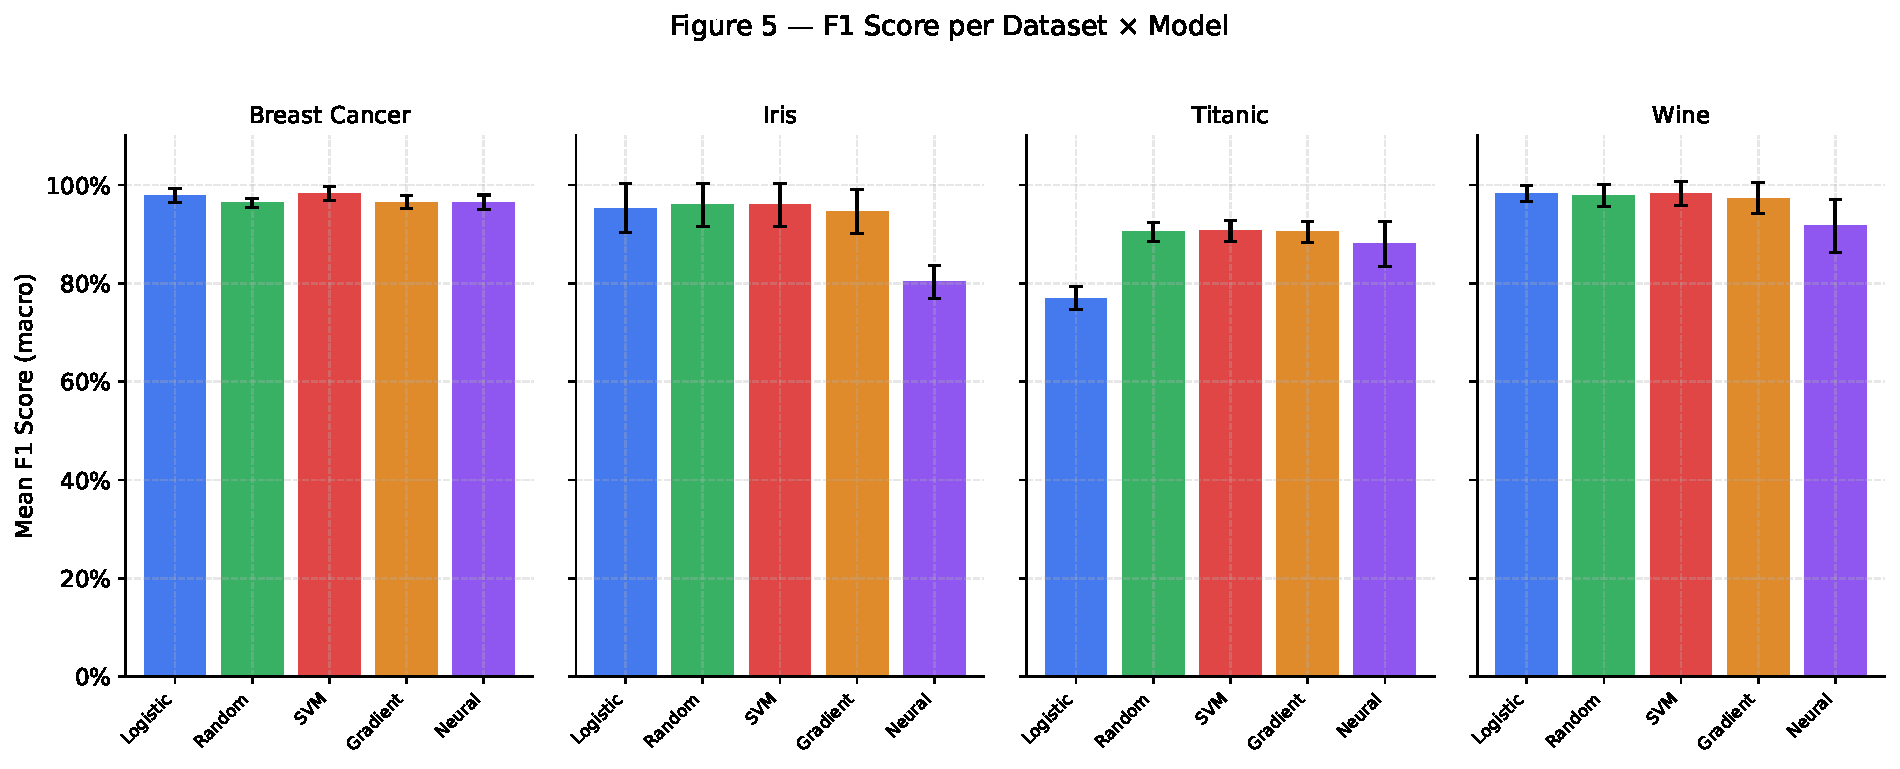
\includegraphics[width=\linewidth]{../figures/fig5_f1_comparison.pdf}
  \caption{Macro-F1 per dataset and model. Consistent pattern: Neural Network 
  underperforms classical methods across all four datasets.}
  \label{fig:f1}
\end{figure}

\section{Full Results Table}

\begin{table}[h]
\centering
\caption{Full mean ± std across 5 folds. BC = Breast Cancer.}
\label{tab:full}
\small
\begin{tabular}{llccc}
\toprule
\textbf{Dataset} & \textbf{Model} & \textbf{Accuracy} & \textbf{F1} & \textbf{Train(s)} \\
\midrule
\multirow{5}{*}{Iris}
  & Logistic Reg.  & 0.953$\pm$.032 & 0.953$\pm$.032 & 0.004 \\
  & SVM (RBF)      & 0.960$\pm$.033 & 0.960$\pm$.033 & 0.003 \\
  & Random Forest  & 0.960$\pm$.040 & 0.960$\pm$.040 & 0.711 \\
  & Grad. Boosting & 0.947$\pm$.049 & 0.946$\pm$.050 & 0.514 \\
  & Neural Net     & 0.813$\pm$.072 & 0.803$\pm$.082 & 0.070 \\
\midrule
\multirow{5}{*}{Wine}
  & Logistic Reg.  & 0.983$\pm$.021 & 0.983$\pm$.021 & 0.035 \\
  & SVM (RBF)      & 0.983$\pm$.021 & 0.983$\pm$.022 & 0.012 \\
  & Random Forest  & 0.978$\pm$.022 & 0.978$\pm$.022 & 0.707 \\
  & Grad. Boosting & 0.972$\pm$.016 & 0.973$\pm$.016 & 0.652 \\
  & Neural Net     & 0.915$\pm$.038 & 0.917$\pm$.037 & 0.069 \\
\midrule
\multirow{5}{*}{BC}
  & Logistic Reg.  & 0.974$\pm$.013 & 0.979$\pm$.011 & 0.023 \\
  & SVM (RBF)      & 0.977$\pm$.013 & 0.982$\pm$.011 & 0.013 \\
  & Random Forest  & 0.954$\pm$.015 & 0.964$\pm$.013 & 0.741 \\
  & Grad. Boosting & 0.956$\pm$.015 & 0.965$\pm$.013 & 0.859 \\
  & Neural Net     & 0.954$\pm$.013 & 0.965$\pm$.011 & 0.146 \\
\midrule
\multirow{5}{*}{Titanic}
  & Logistic Reg.  & 0.772$\pm$.009 & 0.770$\pm$.009 & 0.003 \\
  & SVM (RBF)      & 0.908$\pm$.010 & 0.907$\pm$.010 & 0.028 \\
  & Random Forest  & 0.906$\pm$.012 & 0.905$\pm$.012 & 0.939 \\
  & Grad. Boosting & 0.906$\pm$.010 & 0.905$\pm$.010 & 0.512 \\
  & Neural Net     & 0.880$\pm$.013 & 0.880$\pm$.013 & 0.234 \\
\bottomrule
\end{tabular}
\end{table}

\end{document}
